\section{Triple Integrals in Cylindrical and Spherical Coordinates} \label{S:11.8.Triple_Integrals_Cylindrical_Spherical}

\vspace*{-14 pt}
\framebox{\hspace*{3 pt}
\parbox{6.25 in}{\begin{goals}
\item What are the cylindrical coordinates of a point, and how are they related to Cartesian coordinates?
\item What is the volume element in cylindrical coordinates? How does this inform us about evaluating a triple integral as an iterated integral in cylindrical coordinates?
\item What are the spherical coordinates of a point, and how are they related to Cartesian coordinates?
\item What is the volume element in spherical coordinates? How does this inform us about evaluating a triple integral as an iterated integral in spherical coordinates?
\end{goals}} \hspace*{3 pt}}

\subsection*{Introduction}

We have encountered two different coordinate systems in $\R^2$ -- the rectangular and polar coordinates systems -- and seen how in certain situations, polar coordinates form a convenient alternative.  In a similar way, there there turn out to be two additional natural coordinate systems in $\R^3$.  Given that we are already familiar with the Cartesian coordinate system for $\R^3$,  we next investigate the cylindrical and spherical coordinate systems (each of which builds upon polar coordinates in $\R^2$).  In what follows, we will see how to convert among the different coordinate systems, how to evaluate triple integrals using them, and some situations in which these other coordinate systems prove advantageous.

\begin{pa} \label{PA:11.8}  In the following questions, we investigate the two new coordinate systems that are the subject of this section:  cylindrical and spherical coordinates.  Our goal is to consider some examples of how to convert from rectangular coordinates to each of these systems, and vice versa.  Triangles and trigonometry prove to be particularly important.
\begin{figure}[ht]
\begin{center}
\begin{minipage}{2.5in}
\begin{center}
%\resizebox{!}{2.4in}{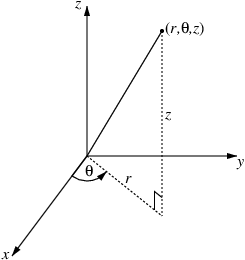
\includegraphics{11_8_Cylindrical_coords}}
  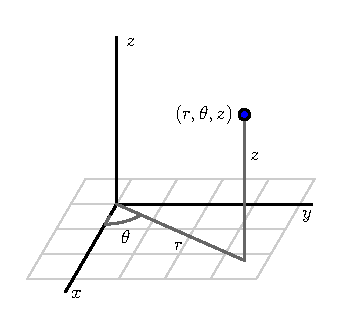
\includegraphics{figures/fig_11_8_cylindrical.eps}
\end{center}
\caption{The cylindrical coordinates of a point.}
\label{F:11.8.Cylindrical_coords}
\end{minipage} \hspace{0.5in}
\begin{minipage}{2.5in}
\begin{center}
%\resizebox{!}{2.4in}{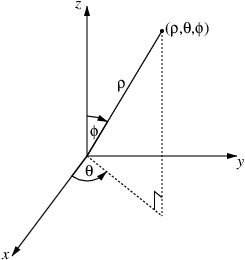
\includegraphics{11_8_Spherical_coords}}
  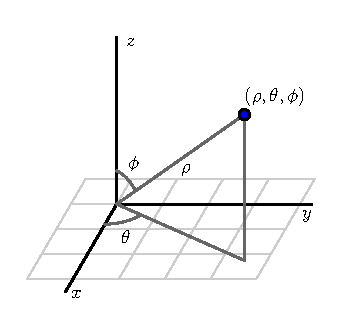
\includegraphics{figures/fig_11_8_spherical.eps}
\end{center}
\caption{The spherical coordinates of a point.}
\label{F:11.8.Spherical_coords}
\end{minipage}
\end{center}
\end{figure}

\noindent The cylindrical coordinates of a point in $\R^3$ are given by $(r,\theta,z)$ where $r$ and $\theta$ are the polar coordinates of the point $(x, y)$ and $z$ is the same $z$ coordinate as in Cartesian coordinates. An illustration is given in Figure \ref{F:11.8.Cylindrical_coords}.
    \begin{enumerate}
    \item[(a)] Find cylindrical coordinates for the point whose Cartesian coordinates are $(-1, \sqrt{3}, 3)$. Draw a labeled picture illustrating all of the coordinates.


	\item[(b)] Find the Cartesian coordinates of the point whose cylindrical coordinates are $\left(2, \frac{5\pi}{4}, 1\right)$. Draw a labeled picture illustrating all of the coordinates.	

	\end{enumerate}

\noindent The spherical coordinates of a point in $\R^3$ are $\rho$ (rho), $\theta$, and $\phi$ (phi), where $\rho$ is the distance from the point to the origin, $\theta$ has the same interpretation it does in polar coordinates, and $\phi$ is the angle between the positive $z$ axis and the vector from the origin to the point, as illustrated in Figure \ref{F:11.8.Spherical_coords}.  \\

\noindent For the following questions, consider the point $P$ whose Cartesian coordinates are $(-2,2,\sqrt{8})$.

\begin{enumerate}
     \item[(c)] What is the distance from $P$ to the origin?  Your result is the value of $\rho$ in the spherical coordinates of $P$.


     \item[(d)] Determine the point that is the projection of $P$ onto the $xy$-plane.  Then, use this projection to find the value of $\theta$ in the polar coordinates of the projection of $P$ that lies in the plane.  Your result is also the value of $\theta$ for the spherical coordinates of the point.



     \item[(e)] Based on the illustration in Figure \ref{F:11.8.Spherical_coords}, how is the angle $\phi$ determined by $\rho$ and the $z$ coordinate of $P$? Use a well-chosen right triangle to find the value of $\phi$, which is the final component in the spherical coordinates of $P$. Draw a carefully labeled picture that clearly illustrates the values of $\rho$, $\theta$, and $\phi$ in this example, along with the original rectangular coordinates of $P$.


     \item[(f)] Based on your responses to (c), (d), and (e), if we are given the Cartesian coordinates $(x,y,z)$ of a point $Q$, how are the values of $\rho$, $\theta$, and $\phi$ in the spherical coordinates of $Q$ determined by $x$, $y$, and $z$?

     

    \end{enumerate}

\end{pa} 

\begin{activitySolution} 

    \ba
    \item We know the $z$ coordinate is $3$. We also know that
\[r = \sqrt{(-1)^2 + (\sqrt{3})^2} = 2 \ \ \ \text{ and } \ \ \ \tan(\theta) = -\sqrt{3}.\]
Since the point $(-1,\sqrt{3})$ is in the second quadrant, we have $\theta = \frac{2\pi}{3}$. So a set of cylindrical coordinates for the point with Cartesian coordinates $(-1, \sqrt{3}, 3)$ is $\left(2, \frac{2\pi}{3}, 3\right)$.

	
	\item In this case we have $x = 2\cos\left(\frac{5\pi}{4}\right) = -\sqrt{2}$, $y =2\sin\left(\frac{5\pi}{4}\right) = -\sqrt{2}$, and $z=1$. 


    \item The distance from $P$ to the origin is
\[\rho = \sqrt{2^2+2^2+(\sqrt{8})^2} = 4.\]

     \item  The projection of the point onto the $xy$-plane is the point $(-2,2,0)$. So $\theta$ satisfies $\tan(\theta) = \frac{-2}{2}=-1$. Since this point is in the second quadrant we have $\theta = \frac{3\pi}{4}$.

     \item Here we have $\cos(\phi) = \frac{z}{\rho} = \frac{\sqrt{8}}{4} = \sqrt{2}{2}$. So $\phi = \frac{\pi}{4}$. Thus, spherical coordinates of the point $P$ are $\left(4, \frac{3\pi}{4}, \frac{\pi}{4}\right)$.  

     \item If we know the Cartesian coordinates $(x,y,z)$ of a point, then spherical coordinates $(\rho, \theta, \phi)$ of this point satisfy
\[\rho :=\sqrt{x^2+y^2+z^2}, \ \ \ \tan(\theta) = \frac{y}{x} \text{ provided } x\neq 0, \ \ \ \text{ and } \ \ \ \cos(\phi) = \frac{z}{\rho} \text{ provided } \rho \neq 0.\]

	\ea

\end{activitySolution}


\afterpa 

\subsection*{Cylindrical Coordinates}

As we stated in Preview Activity~\ref{PA:11.8}, the cylindrical coordinates\index{cylindrical coordinates} of a point are $(r,\theta,z)$, where $r$ and $\theta$ are the polar coordinates of the point $(x, y)$, and $z$ is the same $z$ coordinate as in Cartesian coordinates.  The general situation is illustrated Figure \ref{F:11.8.Cylindrical_coords}.

Since we already know how to convert between rectangular and polar coordinates in the plane, and the $z$ coordinate is identical in both Cartesian and cylindrical coordinates, the conversion equations between the two systems in $\R^3$ are essentially those we found for polar coordinates:
\[x = r \cos(\theta) \hspace{0.25in} y = r \sin(\theta) \hspace{0.25in} z = z\]
\[r^2  = x^2  + y^2 \hspace{0.25in} \tan(\theta) = \frac{y}{x} \hspace{0.25in} z = z.\]
%The reason that the $(r,\theta,z)$ coordinates are called cylindrical coordinates can be seen in the next activity.

Just as with rectangular coordinates, where we usually write $z$ as a function of $x$ and $y$ to plot the resulting surface, in cylindrical coordinates, we often express $z$ as a function of $r$ and $\theta$.  In the following activity, we explore several basic equations in cylindrical coordinates and the corresponding surface each generates.

\begin{activity} \label{A:11.8.1} In this activity, we graph some surfaces using cylindrical coordinates. To improve your intuition and test your understanding, you should first think about what each graph should look like before you plot it using technology.\footnote{e.g., \url{http://www.math.uri.edu/~bkaskosz/flashmo/cylin/} -- to plot $r=2$, set $r$ to 2, $\theta$ to $s$, and $z$ to $t$ -- to plot $\theta = \pi/3$, set $\theta = \pi/3$, $r=s$, and $z=t$, for example. Thanks to Barbara Kaskosz of URI and the Flash and Math team.}
    \ba
    \item Plot the graph of the cylindrical equation $r=2$, where we restrict the values of $\theta$ and $z$ to the intervals  $0 \leq \theta \leq 2\pi$ and $0 \leq z \leq 2$. What familiar shape does the resulting surface take?  How does this example suggest that we call these coordinates \emph{cylindrical coordinates}?



    \item Plot the graph of the cylindrical equation $\theta=2$, where we restrict the other variables to the values $0 \leq r \leq 2$ and $0 \leq z \leq 2$. What familiar surface results?



    \item Plot the graph of the cylindrical equation $z=2$, using $0 \leq \theta \leq 2\pi$ and $0 \leq r \leq 2$. What does this surface look like?



    \item Plot the graph of the cylindrical equation $z=r$, where $0 \leq \theta \leq 2\pi$ and $0 \leq r \leq 2$. What familiar surface results?



    \item Plot the graph of the cylindrical equation $z= \theta$ for $0 \leq \theta \leq 4 \pi$. What does this surface look like?



    \ea

\end{activity}
\begin{smallhint}

\end{smallhint}
\begin{bighint}

\end{bighint}
\begin{activitySolution}
    \ba
    \item In polar coordinates, the graph of $r=2$ is a circle centered at the origin with radius 2. Extending this to cylindrical coordinates, we obtain a cylinder centered at the origin of radius 2, with base on the $xy$-plane and height 2. 

    \item In polar coordinates, the graph of $\theta = 2$ is a line through the origin making an angle of 2 radians with the positive $x$-axis. Extending this to cylindrical coordinates, the graph of $\theta=2$ is a plane through the origin perpendicular to the $xy$-plane making an angle of 2 radians with the $xz$-plane. 

    \item The graph of $z=2$ is just a plane parallel to the $xy$-plane at a distance 2 above the $xy$-plane. With $0 \leq \theta \leq 2\pi$ and $0 \leq r \leq 2$, the graph of $z=2$ is just a disk of radius 2 centered at $(0,0,2)$ within the plane $z=2$. 


    \item For a fixed value of $r$, the graph of $z=r$ and $0 \leq \theta \leq 2\pi$ is a circle of radius $r$ in the plane $z=r$. As $r$ increases the radii increase, so we will obtain a cone with base at the origin, opening up with height $2$. 

    \item For a fixed $\theta$, the graph of $z=\theta$ is a line in the $z = \theta$ plane making an angle of $\theta$ with the $xz$-plane. Allowing $\theta$ to vary will produce a set of lines, spiraling upward so that the result looks like a bit of an auger. 

    \ea
\end{activitySolution}
\aftera


As the name and Activity \ref{A:11.8.1} suggest, cylindrical coordinates are useful for describing surfaces that are cylindrical in nature.

\subsection*{Triple Integrals in Cylindrical Coordinates}

To evaluate a triple integral $\ds \iiint_S f(x,y,z) \, dV$ as an iterated integral in Cartesian coordinates, we use the fact that the volume element $dV$ is equal to $dz \, dy \, dx$ (which corresponds to the volume of a small box). To evaluate a triple integral in cylindrical coordinates, we similarly must understand the volume element $dV$ in cylindrical coordinates.

\begin{activity} \label{A:11.8.2} A picture of a cylindrical box, 
$B = \{(r,\theta,z) : r_1 \leq r \leq r_2, \theta_1 \leq \theta \leq \theta_2, z_1 \leq z \leq z_2\},$
is shown in Figure \ref{F:11.8.Cylindrical_Vol_Element}. Let $\Delta r = r_2-r_1$, $\Delta \theta = \theta_2 - \theta_1$, and $\Delta z = z_2-z_1$. We want to determine the volume $\Delta V$ of $B$ in terms of $\Delta r$, $\Delta \theta$, $\Delta z$, $r$, $\theta$, and $z$.
\begin{figure}[ht]
\begin{center}
%\resizebox{!}{2.5in}{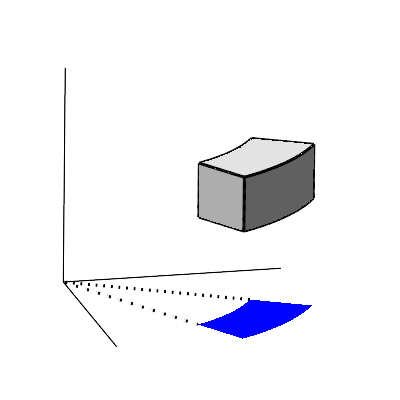
\includegraphics[trim=1.0cm 1.5cm 1.0cm 1.5cm, clip]{11_8_Cylindrical_volume_element}}
  
\includegraphics{figures/fig_11_8_cylindrical_box.eps}
\end{center}
\caption{A cylindrical box.}
\label{F:11.8.Cylindrical_Vol_Element}
\end{figure}
%crop graphics in animate trim=<left> <bottom> <right> <top>, clip with includegraphics

    \ba
    \item Appropriately label $\Delta r$, $\Delta \theta$, and $\Delta z$ in Figure \ref{F:11.8.Cylindrical_Vol_Element}.



    \item Let $\Delta A$ be the area of the projection of the box, $B$, onto the $xy$-plane, which is shaded blue in Figure \ref{F:11.8.Cylindrical_Vol_Element}.  Recall that we previously determined the area $\Delta A$ in polar coordinates in terms of $r$, $\Delta r$, and $\Delta \theta$. In light of the fact that we know $\Delta A$ and that $z$ is the standard $z$ coordinate from Cartesian coordinates, what is the volume $\Delta V$ in cylindrical coordinates?



    \ea


\end{activity}
\begin{smallhint}

\end{smallhint}
\begin{bighint}

\end{bighint}
\begin{activitySolution}
    \ba
    \item The labels are shown below. 
\begin{center}
\resizebox{!}{2.5in}{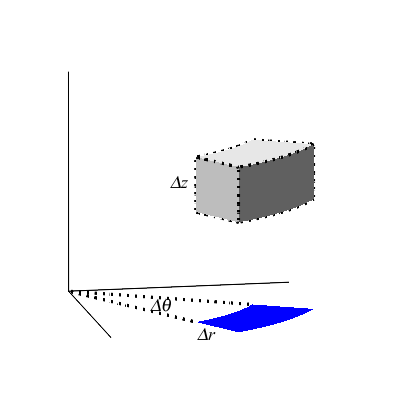
\includegraphics[trim=1.0cm 1.5cm 1.0cm 1.5cm, clip]{11_8_cbox_labels}}
\end{center}

    \item Recall that $\Delta A$ was $\frac{1}{2}(r_{i+1}+r_i) \Delta r \ \Delta \theta$. Since $z$ is just the standard height, we have 
\[\Delta V = \Delta A \ \Delta z = \frac{1}{2}(r_{i+1}+r_i) \Delta r \ \Delta \theta \Delta z.\]

    \ea
\end{activitySolution}
\aftera



Activity \ref{A:11.8.2} demonstrates that the volume element $dV$ in cylindrical coordinates is given by $dV = r \, dz \, dr \, d\theta$, and hence the following rule holds in general.

\vspace*{5pt}
\nin \framebox{\hspace*{3 pt}
\parbox{6.25 in}{Given a continuous function $f = f(x,y,z)$ over a region $S$ in $\R^3$,
$$\ds \iiint_S f(x,y,z) \, dV = \iiint_S f(r\cos(\theta), r\sin(\theta), z) \, r \, dz \, dr \, d\theta.$$
The latter expression is an \textbf{iterated integral in cylindrical coordinates}.\index{iterated integral!cylindrical coordinates}
} \hspace*{3 pt}}
\vspace*{5pt}

Of course, to complete the task of writing an iterated integral in cylindrical coordinates, we need to determine the limits on the three integrals: $\theta$, $r$, and $z$.  In the following activity, we explore how to do this in several situations where cylindrical coordinates are natural and advantageous.

\newpage

\begin{activity} \label{A:11.8.3} In each of the following questions, set up, but do not evaluate, the requested integral expression.

\ba

	\item Let $S$ be the solid bounded above by the graph of $z = x^2+y^2$ and below by $z=0$ on the unit circle. Determine an iterated integral expression in cylindrical coordinates that gives the volume of $S$.

	\item Suppose the density of the cone defined by $r = 1 - z$, with $z \geq 0$, is given by $\delta(r, \theta, z) = z$. A picture of the cone is shown in Figure \ref{F:11.8.Cylindrical_ex}, and the projection of the cone onto the $xy$-plane in given in Figure \ref{F:11.8.Cylindrical_proj}. Set up an iterated integral in cylindrical coordinates that gives the mass of the cone.
\begin{figure}[ht]
\begin{center}
\begin{minipage}{2.5in}
\begin{center}
%\resizebox{!}{2.4in}{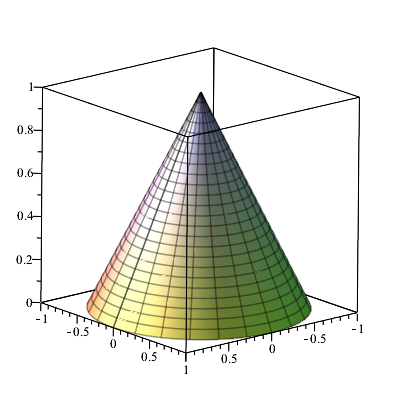
\includegraphics{11_8_Cylindrical_ex}}
  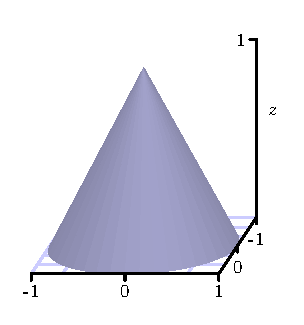
\includegraphics{figures/fig_11_8_cone.eps}
\end{center}
\caption{The cylindrical cone $r = 1-z$.}
\label{F:11.8.Cylindrical_ex}
\end{minipage} \hspace{0.5in}
\begin{minipage}{2.5in}
\begin{center}
%\resizebox{!}{2.4in}{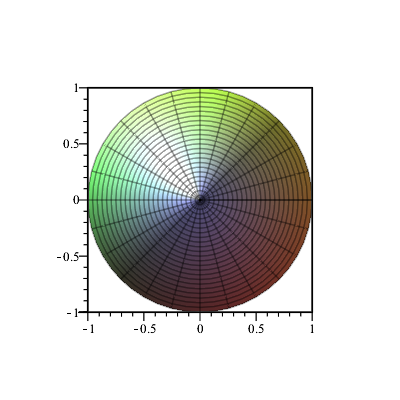
\includegraphics{11_8_Cylindrical_ex_proj}}
  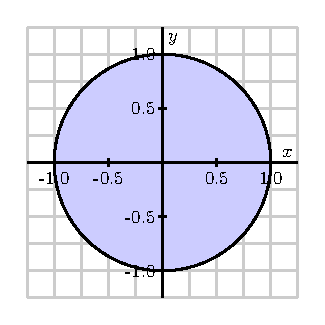
\includegraphics{figures/fig_11_8_cone_project.eps}
\end{center}
\caption{The projection into the $xy$-plane.}
\label{F:11.8.Cylindrical_proj}
\end{minipage}
\end{center}
\end{figure}

	\item Determine an iterated integral expression in cylindrical coordinates whose value is the volume of the solid bounded below by the cone $z = \sqrt{x^2+y^2}$ and above by the cone $z = 4 - \sqrt{x^2+y^2}$. A picture is shown in Figure \ref{F:11.8.Cylindrical_ex2}.
\begin{figure}[ht]
\begin{center}
%\resizebox{!}{2.75in}{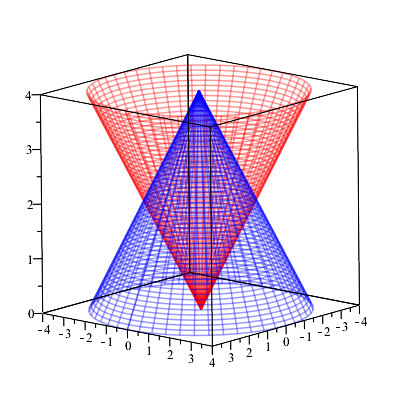
\includegraphics{11_8_Cylindrical_ex2}}
  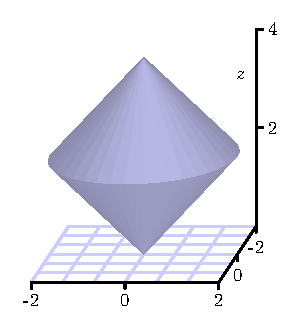
\includegraphics{figures/fig_11_8_two_cones.eps}
\end{center}
\caption{A solid bounded by the cones $z = \sqrt{x^2+y^2}$  and $z = 4 - \sqrt{x^2+y^2}$.}
\label{F:11.8.Cylindrical_ex2}
\end{figure}

\ea

\end{activity}
\begin{smallhint}

\end{smallhint}
\begin{bighint}

\end{bighint}
\begin{activitySolution}

\ba
\item Since $x^2+y^2=r^2$ in cylindrical coordinates, our limits on $z$ will be $0 \leq z \leq r^2$. Thus, an iterated integral in cylindrical coordinates that gives the volume of $S$ is  
\[\int \int \int_S 1 \, dV = \int_{0}^{2\pi} \int_0^1 \int_0^{r^2} (1) r \, dz \, dr \, d\theta.\]
Now
\begin{align*}
\int_{0}^{2\pi} \int_0^1 \int_0^{r^2} r \, dz \, dr \, d\theta &= \int_{0}^{2\pi} \int_0^1 \left. rz \right|_0^{r^2} \, dr \, d\theta \\
	&= \int_{0}^{2\pi} \int_0^1 r^3 \, dr \, d\theta \\
	&= \int_{0}^{2\pi} \left. \frac{r^4}{4} \right|_0^1 \, d\theta \\
	&= \frac{1}{4} \int_{0}^{2\pi} \, d\theta \\
	&= \frac{\pi}{2}.
\end{align*}

\item Recall that mass is the integral of density, so the mass of the cone is
\[\int \int \int_S \delta(r, \theta, z) \, dV.\]
The cone is bounded below by the $xy$-plane and above by the surface $r=1-z$. If we integrate with respect to $z$ first, then the limits on $z$ are $0 \leq z \leq 1-r$. When can project the surface into the $xy$-plane as shown in Figure \ref{F:11.8.Cylindrical_proj} to find the limits on $r$ and $\theta$. Note than when $z=0$ we have $r=1$, so the projection is a circle with radius centered at the origin. Therefore, the mass of the cone given the the iterated integral
\[\int \int \int_S \delta(r, \theta, z) \, dV = \int_0^{2\pi} \int_0^1 \int_0^{1-r} zr \, dz \, dr \, d\theta.\]

\item In cylindrical coordinates the cones are $z=r$ and $z=4-r$. So we have $r \leq z \leq 4-r$. Now $z=r$ and $z=4-r$ intersect when $r = 4-r$ or when $r=2$. So the projection of this solid in the $xy$-plane is the disk $0 \leq r \leq 2$ and $0 \leq \theta \leq 2\pi$. So an iterated integral in cylindrical coordinates that gives the volume of this solid is
\[\int_0^{2\pi} \int_0^2 \int_{r}^{4-r} r \, dz \, dr \, d\theta.\]

\ea

\end{activitySolution}
\aftera


\subsection*{Spherical Coordinates}

As we saw in Preview Activity~\ref{PA:11.8}, the spherical coordinates\index{spherical coordinates} of a point in 3-space have the form $(\rho, \theta, \phi)$, where $\rho$ is the distance from the point to the origin, $\theta$ has the same meaning as in polar coordinates, and $\phi$ is the angle between the positive $z$ axis and the vector from the origin to the point.  The overall situation is  illustrated in Figure \ref{F:11.8.Spherical_coords}.

\begin{figure}[ht]
\begin{center}
%\resizebox{!}{2.75in}{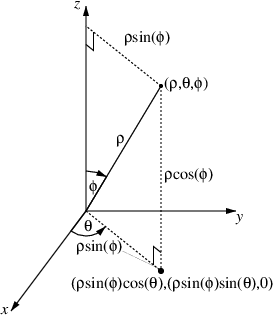
\includegraphics{11_8_Spherical_to_Cartesian}}
  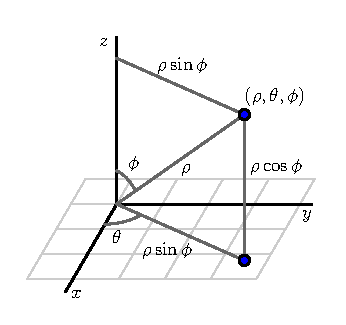
\includegraphics{figures/fig_11_8_spherical_explain.eps}
\end{center}
\caption{Converting from spherical to Cartesian coordinates.}
\label{F:11.8.Spherical_to_Cartesian}
\end{figure}

The example in Preview Activity \ref{PA:11.8} suggests that given a point in rectangular coordinates, $(x,y,z)$, we can find the corresponding spherical coordinates.  Indeed, this holds generally by using the relationships
\[\rho  = \sqrt{x^2  + y^2 + z^2}  \hspace{0.25in} \tan(\theta) = \frac{y}{x}  \hspace{0.25in} \cos(\phi) = \frac{z}{\rho} \]
where in the latter two equations, we require $x \ne 0$ and $\rho \ne 0$.

To convert from given spherical coordinates to Cartesian coordinates, we use the equations 
\[x = \rho \sin(\phi) \cos(\theta) \hspace{0.25in} y = \rho \sin(\phi) \sin(\theta) \hspace{0.25in} z = \rho \cos(\phi),\]
as illustrated in Figure~\ref{F:11.8.Spherical_to_Cartesian}.

%\begin{activity} \label{A:11.8.6} 
\ba
	\item Find a set of spherical coordinates of the point whose Cartesian coordinates are $(-1, 1, 1)$. Draw a picture to illustrate all of the coordinates.
	
	
	
	\item Find the Cartesian coordinates of the point whose spherical coordinates are $(\rho, \theta, \phi) = \left(2, \frac{\pi}{6}, \frac{\pi}{3}\right)$. Draw a picture to illustrate all of the coordinates.
	
	
	
	\ea

\end{activity}
\begin{smallhint} 

\end{smallhint}
\begin{bighint}

\end{bighint}
\begin{activitySolution}
\ba
	\item We have $\rho = \sqrt{(-1)^2+1^2+1^2} = \sqrt{3}$, $\tan(\theta) = -1$, and $\cos(\phi) = \frac{1}{\sqrt{3}}$. Since $(-1,1)$ is in the second quadrant, we have $\theta = \frac{3\pi}{4}$, and the value of $\phi$ is $\arccos\left(\frac{1}{\sqrt{3}}\right) \approx 0.955$.  So $\left(\frac{1}{\sqrt{3}}, \frac{3\pi}{4}, \arccos\left(\frac{1}{\sqrt{3}}\right)\right)$ is a set of spherical coordinates of the point whose Cartesian coordinates are $(-1, 1, 1)$, as illustrated in the figure below. 
\begin{center}
\resizebox{!}{2.0in}{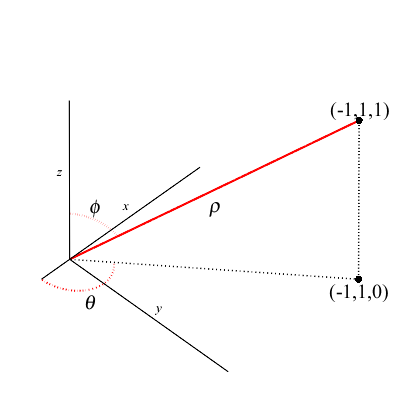
\includegraphics{11_8_spherical_1}}
\end{center}	
	
	
	\item Translating spherical coordinates to Cartesian coordinates we have 
\begin{align*}
x &= 2 \sin\left(\frac{\pi}{3}\right)\cos\left(\frac{\pi}{6}\right) = \frac{3}{2} \\
y &= 2 \sin\left(\frac{\pi}{3}\right)\sin\left(\frac{\pi}{6}\right) = \frac{\sqrt{3}}{2} \\
z &= 2 \cos\left(\frac{\pi}{3}\right) = 1.
\end{align*}
So the Cartesian coordinates of the point whose spherical coordinates are $\left(2, \frac{\pi}{6}, \frac{\pi}{3}\right)$ are $\left(\frac{3}{2}, \frac{\sqrt{3}}{2}, 1\right)$ as illustrated below. 
\begin{center}
\resizebox{!}{2.0in}{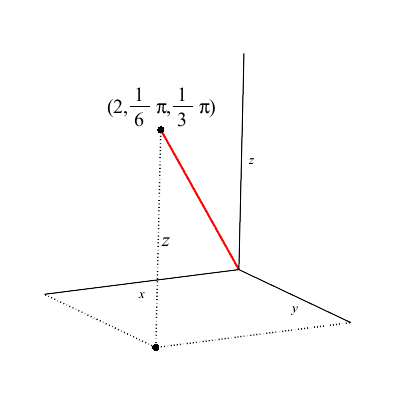
\includegraphics{11_8_spherical_2}}
\end{center}	
	
	
	
	\ea
\end{activitySolution}
\aftera


When it comes to thinking about particular surfaces in spherical coordinates, similar to our work with cylindrical and Cartesian coordinates, we usually write $\rho$ as a function of $\theta$ and $\phi$; this is a natural analog to polar coordinates, where we often think of our distance from the origin in the plane as being a function of $\theta$.  In spherical coordinates, we likewise often view $\rho$ as a function of $\theta$ and $\phi$, thus viewing distance from the origin as a function of two key angles.  

In the following activity, we explore several basic equations in spherical coordinates and the surfaces they generate.

\begin{activity} \label{A:11.8.7} In this activity, we graph some surfaces using spherical coordinates. To improve your intuition and test your understanding, you should first think about what each graph should look like before you plot it using technology.\footnote{e.g., \url{http://www.flashandmath.com/mathlets/multicalc/paramsphere/surf_graph_sphere.html} -- to plot $\rho=2$, set $\rho$ to 2, $\theta$ to $s$, and $\phi$ to $t$, for example. Thanks to Barbara Kaskosz of URI and the Flash and Math team.}
    \ba
    \item Plot the graph of $\rho = 1$, where $\theta$ and $\phi$ are restricted to the intervals  $0 \leq \theta \leq 2\pi$ and $0 \leq \phi \leq \pi$. What is the resulting surface? How does this particular example demonstrate the reason for the name of this coordinate system?

    \item Plot the graph of $\phi = \frac{\pi}{3}$, where $\rho$ and $\theta$ are restricted to the intervals $0 \leq \rho \leq 1$ and $0 \leq \theta \leq 2\pi$. What familiar surface results?

    \item Plot the graph of $\theta = \frac{\pi}{6}$, for $0 \leq \rho \leq 1$ and $0 \leq \phi \leq \pi$. What familiar shape arises?

    \item Plot the graph of $\rho = \theta$, for $0 \leq \phi \leq \pi$ and $0 \leq \theta \leq 2 \pi$. How does the resulting surface appear?



    \ea

\end{activity}
\begin{smallhint}

\end{smallhint}
\begin{bighint}

\end{bighint}
\begin{activitySolution}
    \ba
    \item Since $\rho$ measures the distance from the origin to a point, the graph of $\rho = 1$ is the set of all points that are a distance 1 from the origin. This makes $\rho=1$ the equation of the sphere of radius 1 centered at the origin. 

    \item All points with $\phi = \frac{\pi}{3}$ are at a fixed angle from the positive $z$-axis. The set of such points with $0 \leq \rho \leq 1$ is a cone making an angle of $\frac{\pi}{3}$ with the positive $z$-axis having a slant height of 1. 

    \item As in cylindrical coordinates, the graph of $\theta = 2$ is a plane through the origin perpendicular to the $xy$-plane making an angle of 2 radians with the $xz$-plane. With $0 \leq \rho \leq 1$ and $0 \leq \phi \leq \pi$, we obtain a semicircle or radius 1 centered at the origin in this plane.


    \item For a fixed value of $\theta$, the graph of $\rho=\theta$ is an intersection of a sphere of radius $\theta$ centered at the origin with a plane through the origin. If $0 \leq \phi \leq \pi$, then we get a semicircle. As $\theta$ increases from $0$ to $2\pi$, the radii of the semicircles increase, leaving us with a surface that looks like a snail shell. 

    \ea
\end{activitySolution}
\aftera


As the name and Activity \ref{A:11.8.7} indicate, spherical coordinates are particularly useful for describing surfaces that are spherical in nature; they are also convenient for working with certain conical surfaces.

\subsection*{Triple Integrals in Spherical Coordinates}

As with rectangular and cylindrical coordinates, a triple integral $\ds \iiint_S f(x,y,z) \, dV$ in spherical coordinates can be evaluated as an iterated integral once we understand the volume element $dV$.

\begin{activity} \label{A:11.8.8} To find the volume element $dV$ in spherical coordinates, we need to understand how to determine the volume of a spherical box of the form $\rho_1 \leq \rho \leq \rho_2$ (with $\Delta \rho = \rho_2-\rho_1)$, $\phi_1 \leq \phi \leq \phi_2$ (with $\Delta \phi = \phi_2-\phi_1$), and $\theta_1 \leq \theta \leq \theta_2$ (with $\Delta \theta = \theta_2-\theta_1$). An illustration of such a box is given in Figure \ref{F:11.8.Spherical_Vol_Element}. This spherical box is a bit more complicated than the cylindrical box we encountered earlier. In this situation, it is easier to approximate the volume $\Delta V$ than to compute it directly. Here we can approximate the volume $\Delta V$ of this spherical box with the volume of a Cartesian box whose sides have the lengths of the sides of this spherical box. In other words,
       \[\Delta V \approx |PS| \ |\overset{\frown}{PR}| \ |\overset{\frown}{PQ}|,\]
  where $ |\overset{\frown}{PR}|$ denotes the length of the circular arc from $P$ to $R$.
\begin{figure}[ht]
\begin{center}
\begin{minipage}{2.5in}
\begin{center}
%\resizebox{!}{2.4in}{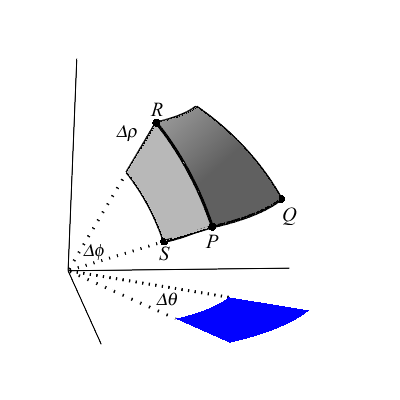
\includegraphics[trim=0.5cm 1cm 1.5cm 1cm, clip]{11_8_Spherical_volume_element}}
  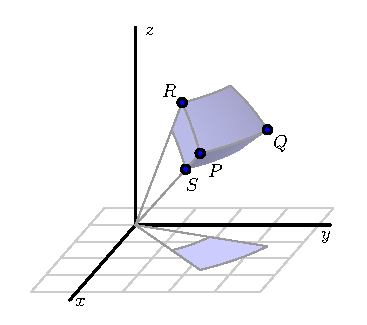
\includegraphics{figures/fig_11_8_spherical_box.eps}
\end{center}
\caption{A spherical box.}
\label{F:11.8.Spherical_Vol_Element}
\end{minipage} \hspace{0.5in}
\begin{minipage}{2.5in}
\begin{center}
%\resizebox{!}{2.4in}{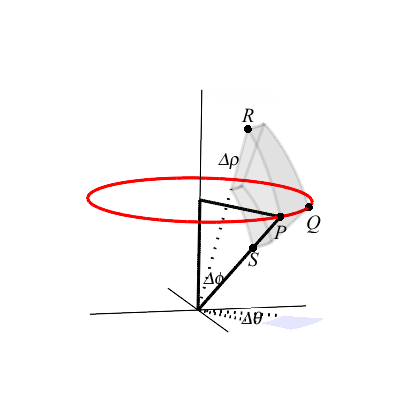
\includegraphics[trim=1.5cm 1.5cm 1.5cm 1.5cm, clip]{11_8_Spherical_volume_element_b}}
  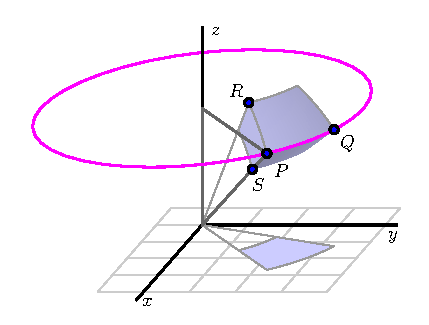
\includegraphics{figures/fig_11_8_spherical_volume.eps}
\end{center}
\caption{A spherical volume element.}
\label{F:11.8.Spherical_Vol_Element_b}
\end{minipage}
\end{center}
\end{figure}
%crop graphics in animate trim=<left> <bottom> <right> <top>, clip with includegraphics
    \ba
        \item What is the length $|PS|$ in terms of $\rho$? 
        %$\Delta \theta$, $\Delta \phi$, $r_1$, $r_2$, $\theta_1$, $\theta_2$, $\phi_1$, and $\phi_2$?

    \item What is the length of the arc $\overset{\frown}{PR}$? (Hint: The arc $\overset{\frown}{PR}$ is an arc of a circle of radius $\rho_2$, and arc length along a circle is the product of the angle measure (in radians) and the circle's radius.)


    \item What is the length of the arc $\overset{\frown}{PQ}$? (Hint: The arc $\overset{\frown}{PQ}$ lies on a horizontal circle as illustrated in Figure \ref{F:11.8.Spherical_Vol_Element_b}. What is the radius of this circle?)


    \item Use your work in (a), (b), and (c) to determine an approximation for $\Delta V$ in spherical coordinates.


    \ea

\end{activity}
\begin{smallhint}

\end{smallhint}
\begin{bighint}

\end{bighint}
\begin{activitySolution}
   \ba
    \item The length $|PS|$ is just $\Delta \rho$. 

    \item This arc is a fraction $\frac{\Delta \phi}{2 \pi}$ of the entire circle of radius $\rho_2$, so its length is
\[\left(\frac{\Delta \phi}{2\pi}\right)(2 \pi \rho_2) = \rho_2 \Delta \phi.\]


    \item The radius of the on which the arc $\overset{\frown}{PQ}$ lies is $\rho_2 \sin(\phi_2)$, so the length of the arc $\overset{\frown}{PQ}$ is  \[\left(\frac{\Delta \theta}{2\pi}\right)(2 \pi \rho_2 \sin(\phi_2)) = \rho_2 \sin(\phi_2) \Delta \theta.\]


    \item The results from the previous parts of this activity show that
\[\Delta V \approx \rho_2^2 \sin(\phi_2) \Delta \rho \Delta \phi \Delta \theta.\]
Letting $\Delta \rho$, $\Delta \phi$, and $\Delta \theta$ go to 0 gives us
\[dV = \rho^2 \sin(\phi) \, d\rho \, d\phi \, d\theta.\]

    \ea
\end{activitySolution}
\aftera



Letting $\Delta \rho$, $\Delta \phi$ and $\Delta \theta$ go to 0, it follows from the final result in
Activity \ref{A:11.8.8} that\\ $dV = \rho^2 \, \sin(\phi) \, d\rho \, d\phi \, d\theta$ in spherical coordinates, and thus allows us to state the following general rule.

\vspace*{5pt}
\nin \framebox{\hspace*{3 pt}
\parbox{6.25 in}{Given a continuous function $f = f(x,y,z)$ over a region $S$ in $\R^3$,
$$\iiint_S f(x,y,z) \, dV = \iiint_S f(\rho\sin(\phi)\cos(\theta), \rho \sin(\phi) \sin(\theta), \rho \cos(\phi)) \, \rho^2 \sin(\phi) \, d\rho \, d\phi \, d\theta.$$
The latter expression is an \textbf{iterated integral in spherical coordinates}\index{iterated integral!spherical coordinates}.
} \hspace*{3 pt}}
\vspace*{5pt}

Finally, in order to actually evaluate an iterated integral in spherical coordinates, we must of course determine the limits of integration in $\theta$, $\phi$,  and $\rho$.  The process is similar to our earlier work in the other two coordinate systems.

%\begin{activity} \label{A:11.8.9} We can use spherical coordinates to derive the formula for the volume of a sphere of radius $a$.
    \ba
    \item How can we describe a sphere in spherical coordinates? (Hint: Refer to Activity \ref{A:11.8.7}, part (a).)



    \item Use the result of (a) to set up and evaluate an iterated integral in spherical coordinates to find the volume of a sphere of radius $a$.


    \ea

\end{activity}
\begin{smallhint}

\end{smallhint}
\begin{bighint}

\end{bighint}
\begin{activitySolution}
\ba
\item A sphere of radius $a$ in spherical coordinates can be represented by $\rho=a$ for $0 \leq \phi \leq \pi$ and $0 \leq \theta \leq 2\pi$. 

\item Recall that the volume of a solid $S$ is given by
\[\int \int \int_S \, dV.\]
Thus, the volume of a sphere of radius $a$ can be calculated as an iterated integral as follows:
\begin{align*}
\int \int \int_S \, dV &= \int_0^{2\pi} \int_0^{\pi} \int_0^{a} \rho^2 \sin(\phi) \, d\rho \, d\phi \, d\theta \\
	&= \int_0^{2\pi} \int_0^{\pi} \left. \left[\frac{\rho^3}{3} \sin(\phi) \right]\right|_0^a  \, d\phi \, d\theta \\
	&= \int_0^{2\pi} \int_0^{\pi} \frac{a^3}{3} \sin(\phi) \, d\phi \, d\theta \\
	&= \int_0^{2\pi} \left. \left[-\frac{a^3}{3} \cos(\phi)\right]\right|_0^{\pi} \, d\theta \\
	&= \int_0^{2\pi} 2\frac{a^3}{3} \, d\theta \\
	&= \frac{4}{3}\pi a^3.
\end{align*}
\ea
\end{activitySolution}
\aftera


\begin{activity} \label{A:11.8.10}  We can use spherical coordinates to help us more easily understand some natural geometric objects.
    \ba
    \item Recall that the sphere of radius $a$ has spherical equation $\rho = a$.  Set up and evaluate an iterated integral in spherical coordinates to determine the volume of a sphere of radius $a$. 
    
    \item Set up, but do not evaluate, an iterated integral expression in spherical coordinates whose value is the mass of the solid obtained by removing the cone $\phi=\frac{\pi}{4}$ from the sphere $\rho = 2$ if the density $\delta$ at the point $(x,y,z)$ is $\delta(x,y,z) = \sqrt{x^2+y^2+z^2}$.  An illustration of the solid is shown in Figure \ref{F:11.8.Spherical_ex2}.
\begin{figure}[ht]
\begin{center}
%\resizebox{!}{2.75in}{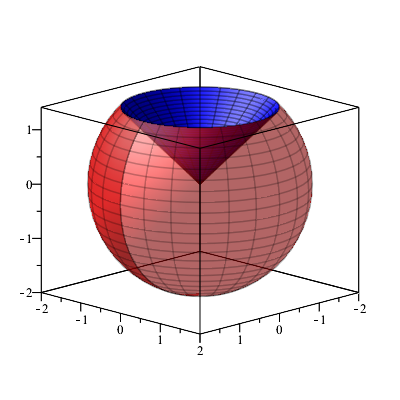
\includegraphics{11_8_Spherical_ex2}}
  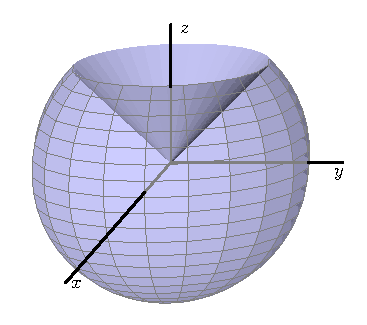
\includegraphics{figures/fig_11_8_sphere_cone.eps}
\end{center}
\caption{The solid cut from the sphere $\rho = 2$ by the cone $\phi=\frac{\pi}{4}$.}
\label{F:11.8.Spherical_ex2}
\end{figure}
    \ea



\end{activity}
\begin{smallhint}

\end{smallhint}
\begin{bighint}

\end{bighint}
\begin{activitySolution}

\ba
\item Recall that the volume of a solid $S$ is given by
\[\int \int \int_S \, dV.\]
Thus, the volume of a sphere of radius $a$ can be calculated as an iterated integral as follows:
\begin{align*}
\int \int \int_S \, dV &= \int_0^{2\pi} \int_0^{\pi} \int_0^{a} \rho^2 \sin(\phi) \, d\rho \, d\phi \, d\theta \\
	&= \int_0^{2\pi} \int_0^{\pi} \left. \left[\frac{\rho^3}{3} \sin(\phi) \right]\right|_0^a  \, d\phi \, d\theta \\
	&= \int_0^{2\pi} \int_0^{\pi} \frac{a^3}{3} \sin(\phi) \, d\phi \, d\theta \\
	&= \int_0^{2\pi} \left. \left[-\frac{a^3}{3} \cos(\phi)\right]\right|_0^{\pi} \, d\theta \\
	&= \int_0^{2\pi} 2\frac{a^3}{3} \, d\theta \\
	&= \frac{4}{3}\pi a^3.
\end{align*}


\item The limits on $\rho$ are $0 \leq \rho \leq 2$ and on $\theta$ are $0 \leq \theta \leq 2\pi$. To account for the cone being removed from the sphere we restrict $\phi$. The cone opens from $\phi = 0$ to $\phi = \frac{\pi}{4}$, so the limits on $\phi$ that remove the cone are $\frac{\pi}{4} \leq \phi \leq \pi$. Therefore, the density of the solid is found by 
\[\int_{0}^{2\pi} \int_{\pi/4}^{\pi} \int_0^2 \rho^3 \sin(\phi) \, d\rho \, d\phi \, d\theta.\]
\ea

\end{activitySolution}
\aftera


\begin{summary}

\item The cylindrical coordinates of a point $P$ are $(r,\theta,z)$ where $r$ is the distance from the origin to the projection of $P$ onto the $xy$-plane, $\theta$ is the angle that the projection of $P$ onto the $xy$-plane makes with the positive $x$-axis, and $z$ is the vertical distance from $P$ to the projection of $P$ onto the $xy$-plane.  When $P$ has rectangular coordinates $(x,y,z)$, it follows that  its cylindrical coordinates are given by
\[r^2  = x^2  + y^2, \hspace{0.25in} \tan(\theta) = \frac{y}{x}, \hspace{0.25in} z = z.\]
When $P$ has given cylindrical coordinates $(r,\theta,z)$, its rectangular coordinates are 
\[x = r \cos(\theta), \hspace{0.25in} y = r \sin(\theta), \hspace{0.25in} z = z.\]
\item The volume element $dV$ in cylindrical coordinates is $dV = r \, dz \, dr \, d\theta$. Hence, a triple integral $\ds \iiint_S f(x,y,z) \, dA$ can be evaluated as the iterated integral
    \[\iiint_S f(r\cos(\theta), r\sin(\theta), z) \, r \, dz \, dr \, d\theta.\]
\item The spherical coordinates of a point $P$ in 3-space are $\rho$ (rho), $\phi$ (phi), and $\theta$, where $\rho$ is the distance from $P$ to the origin, $\phi$ is the angle between the positive $z$ axis and the vector from the origin to $P$, and $\theta$ is the angle that the projection of $P$ onto the $xy$-plane makes with the positive $x$-axis.  When $P$ has Cartesian coordinates $(x,y,z)$, the spherical coordinates are given by
\[\rho^2  = x^2  + y^2 + z^2, \hspace{0.25in} \tan(\theta) = \frac{y}{x}, \hspace{0.25in} \cos(\phi) = \frac{z}{\rho}.\]
Given the point $P$ in spherical coordinates $(\rho, \phi, \theta)$, its rectangular coordinates are 
\[x = \rho \sin(\phi) \cos(\theta), \hspace{0.25in} y = \rho \sin(\phi) \sin(\theta), \hspace{0.25in} z = \rho \cos(\phi).\]
\item The volume element $dV$ in spherical coordinates is $dV = \rho^2 \sin(\phi) \, d\rho \, d\phi \, d\theta$. Thus, a triple integral $\ds \iiint_S f(x,y,z) \, dA$ can be evaluated as the iterated integral
    \[\iiint_S f(\rho\sin(\phi)\cos(\theta), \rho \sin(\phi) \sin(\theta), \rho \cos(\phi)) \, \rho^2 \sin(\phi) \, d\rho \, d\phi \, d\theta.\]
\end{summary}


\nin \hrulefill

\begin{exercises} 

\item In each of the following questions, set up an iterated integral expression whose value determines the desired result.  Then, evaluate the integral first by hand, and then using appropriate technology.
	\ba
	\item Find the volume of the ``cap'' cut from the solid sphere $x^2 + y^2 + z^2 = 4$ by the plane $z=1$, as well as the $z$-coordinate of its centroid.

	\item Find the $x$-coordinate of the center of mass of the portion of the unit sphere that lies in the first octant (i.e., where $x$, $y$, and $z$ are all nonnegative).  Assume that the density of the solid given by $\delta(x,y,z) = \frac{1}{1+x^2+y^2+z^2}$.

	\item Find the volume of the solid bounded below by the $x$-$y$ plane, on the sides by the sphere $\rho=2
$, and above by the cone $\phi = \pi/3$.


	\item Find the $z$ coordinate of the center of mass of the region that is bounded above by the surface $z = \sqrt{\sqrt{x^2 + y^2}}$, on the sides by the cylinder $x^2 + y^2 = 4$, and below by the $x$-$y$ plane.   Assume that the density of the solid is uniform and constant.

	\item Find the volume of the solid that lies outside the sphere $x^2 + y^2 + z^2 = 1$ and inside the sphere $x^2 + y^2 + z^2 = 2z$.

	\ea

\begin{exerciseSolution}
	\ba
	\item In cylindrical coordinates the volume of the solid is  
\begin{align*}
V &= \int_0^{2\pi} \int_0^{2} \int_{1}^{\sqrt{4-r^2}} r \, dz \, dr \, d\theta \\
	&= \int_0^{2\pi} \int_0^{2} rz\biggm|_{1}^{\sqrt{4-r^2}}  \, dr \, d\theta \\
	&= \int_0^{2\pi} \int_0^{2} r\sqrt{4-r^2} - r  \, dr \, d\theta \\
	&= \int_0^{2\pi} \left[-\frac{1}{3}(4-r^2)^{3/2}-\frac{1}{2}r^2\right]\biggm|_0^{2}  \, d\theta \\
	&= \int_0^{2\pi}  \left[-2+\frac{8}{3}\right] \, d\theta \\
	&= \frac{4}{3}\pi.
\end{align*}
The $z$-coordinate of the centroid of this region is 
\begin{align*}
\overline{z} &= \frac{1}{V} \int_0^{2\pi} \int_0^{2} \int_{1}^{\sqrt{4-r^2}} rz \, dz \, dr \, d\theta \\
	&= \frac{3}{8\pi} \int_0^{2\pi} \int_0^{2} rz^2\biggm|_{1}^{\sqrt{4-r^2}}  \, dr \, d\theta \\
	&= \frac{3}{8\pi} \int_0^{2\pi} \int_0^{2} r(4-r^2) - r  \, dr \, d\theta \\
	&= \frac{3}{8\pi} \int_0^{2\pi} \left[\frac{3}{2}r^2- \frac{1}{4}r^4\right]\biggm|_0^{2}  \, d\theta \\
	&= \frac{3}{8\pi} \int_0^{2\pi}  2 \, d\theta \\
	&= \frac{3}{2}.
\end{align*}


	\item Using spherical coordinates we find that the mass of this solid is 
\begin{align*}
M &= \int_{0}^{\pi/2} \int_{0}^{\pi/2} \int_{0}^{1} \frac{\rho^2 \sin(\phi)}{1+\rho^2} \, d\rho \, d\phi \, d\theta \\
	&= \int_{0}^{\pi/2} \int_{0}^{\pi/2} \int_{0}^{1} \sin(\phi)\left(1-\frac{1}{1+\rho^2}\right) \, d\rho \, d\phi \, d\theta \\
	&= \int_{0}^{\pi/2} \int_{0}^{\pi/2}  \sin(\phi)\left(\rho - \arctan(\rho)\right) \biggm|_{0}^{1}  \, d\phi \, d\theta \\
	&= \left(1-\frac{\pi}{4}\right) \int_{0}^{\pi/2} \int_{0}^{\pi/2}  \sin(\phi) \, d\phi \, d\theta \\
	&= \left(1-\frac{\pi}{4}\right)  \int_{0}^{\pi/2} -\cos(\phi)\biggm|_{0}^{\pi/2} \, d\theta \\
	&= \left(1-\frac{\pi}{4}\right)  \int_{0}^{\pi/2} 1 \, d\theta \\
	&= \frac{\pi}{2}\left(1-\frac{\pi}{4}\right).
\end{align*}
Then the $x$-coordinate of the center of mass of this solid is 
\begin{align*}
\overline{x} &= \frac{1}{M} \int_{0}^{\pi/2} \int_{0}^{\pi/2} \int_{0}^{1} \frac{\rho^3 \sin^2(\phi) \cos(\theta)}{1+\rho^2} \, d\rho \, d\phi \, d\theta \\ 	
	 &= \frac{1}{M} \int_{0}^{\pi/2} \int_{0}^{\pi/2} \int_{0}^{1} \sin^2(\phi) \cos(\theta)\left(\rho-\frac{\rho}{1+\rho^2}\right) \, d\rho \, d\phi \, d\theta \\ 	
	 &= \frac{1}{M} \int_{0}^{\pi/2} \int_{0}^{\pi/2}  \sin^2(\phi) \cos(\theta)\left(\frac{1}{2}\rho^2-\frac{1}{2}\ln(1+\rho^2)\right)\biggm|_{0}^{1} \, d\phi \, d\theta \\ 
	 &= \frac{1-\ln(2)}{2M} \int_{0}^{\pi/2} \int_{0}^{\pi/2}  \sin^2(\phi) \cos(\theta) \, d\phi \, d\theta \\ 
	&= \frac{1-\ln(2)}{2M} \int_{0}^{\pi/2} \int_{0}^{\pi/2} \frac{1}{2}(1-\cos(2\phi)) \cos(\theta) \, d\phi \, d\theta \\
	&= \frac{1-\ln(2)}{4M} \int_{0}^{\pi/2}  \left(\phi -\frac{1}{2}\sin(2\phi))\right) \cos(\theta)\biggm|_{0}^{\pi/2} \, d\theta \\
	&= \frac{1-\ln(2)}{4M} \int_{0}^{\pi/2}  \left(\frac{\pi}{2}\right) \cos(\theta) \, d\theta \\
	&= \frac{\pi(1-\ln(2))}{8M}  \sin(\theta)\biggm|_{0}^{\pi/2} \\
	&= \frac{\pi(1-\ln(2))}{8M} \\
	&= \frac{1-\ln(2)}{4-\pi}. 
\end{align*}


	\item Using spherical coordinates we have that the volume of the solid bounded below by the $x$-$y$ plane, on the sides by the sphere $\rho=2
$, and above by the cone $\phi = \pi/3$ is
\begin{align*}
\int_{0}^{2\pi} \int_{0}^{\pi/3} \int_{0}^{2} \rho^2 \sin(\phi) \, d\rho \, d\phi \, d\theta &= \frac{1}{3} \int_{0}^{2\pi} \int_{0}^{\pi/3}  \rho^3 \sin(\phi) \biggm|_{0}^{2} \, d\phi \, d\theta  \\
	&= \frac{8}{3} \int_{0}^{2\pi} \int_{0}^{\pi/3}  \sin(\phi)  \, d\phi \, d\theta  \\
	&= \frac{8}{3} \int_{0}^{2\pi}   -\cos(\phi) \biggm|_{0}^{\pi/3}  \, d\theta  \\
	&= \frac{8}{3} \int_{0}^{2\pi}  \frac{1}{2}  \, d\theta  \\
	&= \frac{8\pi}{3}.
\end{align*}

	\item Let the density of the solid be $k$. Using cylindrical coordinates we have that the mass of the solid is
\begin{align*}
M &= \int_{0}^{2\pi} \int_{0}^{2} \int_{0}^{\sqrt{r}} kr \, dz \, dr \, d\theta \\
	&= k\int_{0}^{2\pi} \int_{0}^{2} rz\biggm|_{0}^{\sqrt{r}} \, dr \, d\theta \\
	&= k\int_{0}^{2\pi} \int_{0}^{2}  r^{3/2} \, dr \, d\theta \\
	&= \frac{2k}{5} \int_{0}^{2\pi} r^{5/2}\biggm|_{0}^{2}  \, d\theta \\
	&= \frac{8k\sqrt{2}}{5} \int_{0}^{2\pi} \, d\theta \\
	&= \frac{16k\sqrt{2}\pi}{5}.
\end{align*}
Then the $z$ coordinate of the center of mass of the solid is 
\begin{align*}
\overline{z} &= \frac{1}{M}  \int_{0}^{2\pi} \int_{0}^{2} \int_{0}^{\sqrt{r}} krz \, dz \, dr \, d\theta \\
	&= \frac{k}{2M} \int_{0}^{2\pi} \int_{0}^{2} rz^2\biggm|_{0}^{\sqrt{r}} \, dr \, d\theta \\
	&= \frac{k}{2M}\int_{0}^{2\pi} \int_{0}^{2}  r^2 \, dr \, d\theta \\
	&= \frac{k}{6M} \int_{0}^{2\pi} r^{3}\biggm|_{0}^{2}  \, d\theta \\
	&= \frac{4k}{3M} \int_{0}^{2\pi} \, d\theta \\
	&= \frac{5}{6\sqrt{2}}.
\end{align*}


	\item The sphere $x^2 + y^2 + z^2 = 2z$ has equation $\rho^2 = 2\rho \cos(\phi)$ or $\rho = 2\cos(\phi)$ in spherical coordinates.  The two spheres intersect when $1 = 2 z$ or when $z = \frac{1}{2}$. If $\rho = 1$ and $z = \frac{1}{2}$, then $\cos(\phi) = \frac{1}{2}$ and $\phi = \frac{\pi}{3}$. So the volume of this solid is  
\begin{align*}
\int_{0}^{2\pi} \int_{0}^{\pi/3} \int_{1}^{2\cos(\phi)} \rho^2 \sin(\phi) \, d\rho \, d\phi \, d\theta &= \frac{1}{3} \int_{0}^{2\pi} \int_{0}^{\pi/3} \rho^3 \sin(\phi)\biggm|_{1}^{2\cos(\phi)} \, d\phi \, d\theta \\
	&= \frac{1}{3} \int_{0}^{2\pi} \int_{0}^{\pi/3} [8\cos^3(\phi) - 1]\sin(\phi) \, d\phi \, d\theta \\
	&= \frac{1}{3} \int_{0}^{2\pi} [-2\cos^4(\phi) + \cos(\phi)]\biggm|_{0}^{\pi/3}   \, d\theta \\
	&= \frac{11}{24} \int_{0}^{2\pi} \, d\theta \\
	&= \frac{11\pi}{12}. 
\end{align*}


	\ea
\end{exerciseSolution}
%	\item Find the $z$-coordinate of the center of mass of the solid that lies between the hemisphere of radius 2 and the hemisphere of radius 1, each of which are bounded below by the plane $z=0$.  Assume that the density of the solid is given by the function $d(x,y,z)=x^2+y^2+z^2$.  Can you find $\overline{x}$ and $\overline{y}$ without integrating?

	
	\item For each of the following questions, (a) sketch the region of integration, (b) change the coordinate system in which the iterated integral is written to one of the remaining two, and (c) evaluate the iterated integral you deem easiest to evaluate by hand.
	
	\ba
		\item $\ds \int_{0}^{1} \int_{0}^{\sqrt{1-x^2}} \int_{\sqrt{x^2 + y^2}}^{\sqrt{2-x^2-y^2}} xy\, dz \, dy \, dx$
		\item $\ds \int_{0}^{\pi/2} \int_{0}^{\pi} \int_{0}^{1} \rho^2 \sin(\phi) \, d\rho \, d\phi \, d\theta$	
		\item $\ds \int_{0}^{2\pi} \int_{0}^{1} \int_{r}^{1} r^2 \cos(\theta) \, dz \, dr \, d\theta$
	\ea

\begin{exerciseSolution}
	\ba
		\item In cylindrical coordinates, an equivalent iterated integral is 
\[\int_{0}^{\pi/2} \int_{0}^{1} \int_{r}^{\sqrt{2-r^2}} r^3 \cos(\theta) \sin(\theta) \, dz \, dr \, d\theta.\]
Evaluating the integral in cylindrical coordinates gives us 
\begin{align*}
\int_{0}^{\pi/2} \int_{0}^{1} \int_{r}^{\sqrt{2-r^2}} & r^3 \cos(\theta) \sin(\theta) \, dz \, dr \, d\theta = \int_{0}^{\pi}{2} \int_{0}^{1}  r^3 \cos(\theta) \sin(\theta)z\biggm|_{r}^{\sqrt{2-r^2}}  \, dr \, d\theta \\
	&= \int_{0}^{\pi/2} \int_{0}^{1}  r^3 \cos(\theta) \sin(\theta)[\sqrt{2-r^2} - r]  \, dr \, d\theta \\
	&= \int_{0}^{\pi/2} \int_{0}^{1}   \cos(\theta) \sin(\theta) r^3\sqrt{2-r^2} \, dr \, d\theta -  \int_{0}^{\pi/2} \int_{0}^{1}   \cos(\theta) \sin(\theta) r^4  \, dr \, d\theta \\
	&= -\frac{1}{2}\int_{0}^{\pi/2} \int_{2}^{1}   \cos(\theta) \sin(\theta) (2-u)\sqrt{u} \, du \, d\theta -  \frac{1}{5} \int_{0}^{\pi/2} \cos(\theta) \sin(\theta) r^5\biggm|_{0}^{1}   \, d\theta \\
	&= -\frac{1}{2}\int_{0}^{\pi/2}  \cos(\theta) \sin(\theta) \left(\frac{4}{3}u^{3/2}-\frac{2}{5}u^{5/2}\right)\biggm|_{2}^{1}  \, d\theta -  \frac{1}{5} \int_{0}^{\pi/2} \cos(\theta) \sin(\theta) r^5\biggm|_{0}^{1}   \, d\theta \\
	&= \left(\frac{8}{15}\sqrt{2}-\frac{7}{15}\right)\int_{0}^{\pi/2}  \cos(\theta) \sin(\theta)   \, d\theta -  \frac{1}{5} \int_{0}^{\pi/2} \cos(\theta) \sin(\theta)  \, d\theta \\
	&= \left(\frac{8}{15}\sqrt{2}-\frac{7}{15}\right) \frac{1}{2}\sin^2(\theta)\biggm|_{0}^{\pi/2}  -  \frac{1}{5}\left(\frac{1}{2}\sin^2(\theta)\biggm|_{0}^{\pi/2} \right) \\
	&= \frac{1}{2} \left(\frac{8}{15}\sqrt{2}-\frac{7}{15}\right)  -  \frac{1}{10}  \\
	&= \frac{4}{15}\sqrt{2}- \frac{1}{3}.
\end{align*}

		\item In rectangular coordinates an equivalent iterated integral is 
\[\int_{0}^{1} \int_{0}^{\sqrt{1-x^2}} \int_{-\sqrt{1-x^2-y^2}}^{\sqrt{1-x^2-y^2}} \, dz \, dy \, dx.\]
Evaluating the integral in spherical coordinates yields
\begin{align*}
\int_{0}^{\pi/2} \int_{0}^{\pi} \int_{0}^{1} \rho^2 \sin(\phi) \, d\rho \, d\phi \, d\theta &= \frac{1}{3} \int_{0}^{\pi/2} \int_{0}^{\pi}  \rho^3 \sin(\phi)\biggm|_{0}^{1} \, d\phi \, d\theta \\
	&= \frac{1}{3} \int_{0}^{\pi/2} \int_{0}^{\pi}  \sin(\phi) \, d\phi \, d\theta \\
	&= \frac{1}{3} \int_{0}^{\pi/2}   -\cos(\phi)\biggm|_{0}^{\pi} \, d\theta \\
	&= \frac{2}{3} \int_{0}^{\pi/2}  \, d\theta \\
	&= \frac{\pi}{3}. 
\end{align*}
	
		\item In rectangular coordinates an equivalent iterated integral is 
\[\int_{-1}^{1} \int_{-\sqrt{1-x^2}}^{\sqrt{1-x^2}} \int_{\sqrt{x^2+y^2}}^{1} x \, dz \, dy \, dx.\]
Evaluating the integral in cylindrical coordinates yields
\begin{align*}
\int_{0}^{2\pi} \int_{0}^{1} \int_{r}^{1} r^2 \cos(\theta) \, dz \, dr \, d\theta &= \int_{0}^{2\pi} \int_{0}^{1}  r^2 \cos(\theta)z\biggm|_{r}^{1} \, dr \, d\theta \\
	&= \int_{0}^{2\pi} \int_{0}^{1}  r^2 \cos(\theta)(1-r) \, dr \, d\theta \\
	&= \int_{0}^{2\pi}  \cos(\theta)\left(\frac{1}{3}r^3 - \frac{1}{4}r^4\right)\biggm|_{0}^{1} \, d\theta \\
	&= \frac{1}{12} \int_{0}^{2\pi}  \cos(\theta) \, d\theta \\
	&= \frac{1}{12}  \sin(\theta)\biggm|_{0}^{2\pi}  \\
	&= 0.
\end{align*}

	\ea
\end{exerciseSolution}

	\item Consider the solid region $S$ bounded above by the paraboloid $z = 16 - x^2 - y^2$ and below by the paraboloid $z = 3x^2 + 3y^2$.
		\ba
			\item Describe parametrically the curve in $\R^3$ in which these two surfaces intersect.
			\item In terms of $x$ and $y$, write an equation to describe the projection of the curve onto the $x$-$y$ plane.
			\item What coordinate system do you think is most natural for an iterated integral that gives the volume of the solid?
			\item Set up, but do not evaluate, an iterated integral expression whose value is average $z$-value of points in the solid region $S$.  
			\item Use technology to plot the two surfaces and evaluate the integral in (c).  Write at least one sentence to discuss how your computations align with your intuition about where the average $z$-value of the solid should fall. 
		\ea

 
%\item What is the volume of the ice cream cone formed by intersecting the cone $z = \sqrt{x^2 + y^2}$ with the hemisphere of radius 1 centered at $(0,0,0)$?  What is the $z$-coordinate of its centroid?  What does the latter problem, which requires triple integrals, suggest? 


\begin{exerciseSolution}
		\ba
			\item Setting $16-x^2-y^2$ equal to $3x^2+3y^2$ yields the equation $x^2+y^2=4$. When $x^2+y^2=4$, we have $z = 12$. This is the circle centered at $(0,0,12)$ with radius 2 in the $z=12$ plane, and has the parameterization $x(t) = 2\cos(t)$, $y(t) = 2\sin(t)$, and $z=12$ for $0 \leq t \leq 2\pi$. 
			\item The projection of this intersection curve onto the $x$-$y$ plane is the circle centered at the origin of radius 2 and has parameterization $x(t) = 2\cos(t)$ and $y(t) = 2\sin(t)$ for $0 \leq t \leq 2\pi$. 
			\item With the projection as a circle and the surfaces defined in terms of $x^2+y^2$, cylindrical coordinates seem a natural choice. 
			\item An iterated integral expression whose value is average $z$-value of points in the solid region $S$. is
\[\frac{\int_{0}^{2\pi} \int_{0}^{2} \int_{3r^2}^{16-r^2} z \, dz \, dr \, d\theta}{\int_{0}^{2\pi} \int_{0}^{2} \int_{3r^2}^{16-r^2} 1 \, dz \, dr \, d\theta}.\]
			\item A computer algebra system says that the average $z$-value of points in the solid region $S$ is $\frac{44}{5} = 8.8$. The surface is a paraboloid with a rounded cap. Cross sections with constant $z$ values are generally larger as the $z$ values increase, with the exception of a rapid decrease in areas near the top. This suggests that the average $z$ value should be more than half-way up the solid. 
		\ea
\end{exerciseSolution}


\end{exercises}
\afterexercises


\clearpage
